\pagestyle{fancy}
\pagenumbering{arabic} 


The desire to create machines capable of thinking accompanies the human kind since the first programmable computer was invented. Nowadays, artificial intelligence (AI) is a thriving field of research that encompasses various disciplines such as computer science, engineering, statistics, neuroscience, biology, with applications that range from automating routine labour, interpreting images, understanding speech, to making diagnoses in medicine.

Problems that are intellectually difficult for humans to tackle, namely those problems that can be described by a list of formal, mathematical rules, are among the easiest for computers to solve. The real challenge to AI is the resolution of tasks relatively easy for people to perform, but hard to describe in formal terms -- problems that we, as human beings, solve intuitively, instinctively -- such as recognizing objects in images. This instinctive \say{intuitions} are drawn from experience: collections of small facts (data) and personal judgments of facts (information)\footnote{One research project that aims at producing completely automated analyses and reports is the \textit{Automatic Statistician} [\texttt{https://automaticstatistician.com}]: the current version of the Automatic Statistician is a system which explores an open-ended space of possible statistical models to discover a good explanation of the data, and then produces a detailed report with figures and natural-language text. The system is based on reasoning over an open-ended collection of nonparametric models using Bayesian inference.}.

One solution to let machines mimic the process of deduction from experience is to hard-code the knowledge about the reality in formal language, allowing the computer to reason using logical inference rules. This approach, called \textbf{knowledge-based} [\cite{Goodfellow-et-al-2016}], is brute-force in nature and not viable in many practical applications.

Therefore, AI systems need to have the ability to \say{build} their own knowledge by extracting information from raw data. This field of research is known as \textbf{machine learning}. However, the performance of this approach crucially depends on the \textit{representation} of data used -- the usual maxim \say{garbage in, garbage out}. Each bit of information included in the representation is called \textbf{feature}. Selecting or extracting features, that form representations, from raw data is a form of art of its own. Often, as an alternative to hand-designed features, machine learning algorithms are used to learn such \textit{representations} besides learning the \textit{mapping} from representations to outputs. This approach is called \textbf{representation leaning} [\cite{Goodfellow-et-al-2016}]. 

Regardless the methodology used to build such features, the aim is often to separate the \textbf{factors of variation} that explain the observed data. In many cases, these factors are not directly observed: \begin{displayquote}
    \say{[...] They may exist as either unobserved objects or unobserved forces [...] constructs in the human mind [...] concepts or abstractions that help us make sense of the rich variability in the data} -- \cite{Goodfellow-et-al-2016}, pp. 4-5
\end{displayquote}
Therefore, extracting representations can be as difficult as solving the original problem. In these cases representation learning comes unhandy. \textbf{Deep learning} (DL) provides a solution by taking a constructionist approach: creating autonomously complex, expressive, representations of the world in terms of simple, more basic, ones. It can be defined as 
\begin{displayquote}
    \say{[...] A form of machine learning that uses hierarchical abstract layers of latent variables to perform pattern matching and prediction} -- \cite{Polson2017}, p. 1
\end{displayquote}

In the statistical literature inputs are often called \textit{predictors} or, more classically, \textit{independent variables}. Outputs are usually referred to as \textit{responses} or, more classically, \textit{dependent variables}. Throughout the thesis these terms are used interchangeably. However, differences between statistics and machine learning are not limited to nomenclature. They truly can be defined as \say{two cultures} [\cite{Breiman2001}]. In the next section we will discover how a different philosophical approach has been the cause of two, sometimes competing and opposite, visions of the world, that with this work we would like to bring closer. 




\section{The Two Cultures} \label{sec:cultures}
In one of its most contended contributions [\cite{Breiman2001}], Leo Breiman states that
\begin{displayquote}
    \say{There are two cultures in the use of statistical modeling to reach conclusions from data. One assumes that the data are generated by a given \textit{stochastic data model}. The other uses \textit{algorithmic models} and treats the data mechanism as unknown. The statistical community has been committed to the almost exclusive use of data models. This commitment has led to irrelevant theory, questionable conclusions, and has kept statisticians from working on a large range of interesting current problems. Algorithmic modeling, both in theory and practice, has developed rapidly in fields outside statistics. It can be used both on large complex data sets and as a more accurate and informative alternative to data modeling on smaller data sets}
\end{displayquote}
Philosophically, one can think of the world as a deterministic chain of causes and effects. Albeit complex, one can believe that there exist, unique, a cause-effect chain that leads to a specific outcome, manifests itself as a fact of our reality. If this is the case, then  an all-mighty intellect could, in theory, be able to trace back each effect to its cause. Chance would not exist. Even if we admit that randomness pervades parts of out reality, we would still be bounded to reason about the complementary deterministic part. Our human nature, its finiteness, limits us twice: first, it limits the scope of investigation to the deterministic component of the real; second, it limits our possibilities to reason directly about it. We are bound to observe the deterministic part of our universe in an indirect way that, alone, creates an additional layer of randomness between us and the \say{truth}. Fortunately, statistics provides us with mathematical tools to deal with this latter layer.

The role of statistics is to try to discover and understand the functioning of our reality starting from collections of facts: the data. These are regarded as being generated by a black box in which a set of possible causes, interpreted as a vector of input variables $x$, enter on one side and an effect, a response variables $y$, comes out on the other:

\begin{figure}[h!]
    \centering
    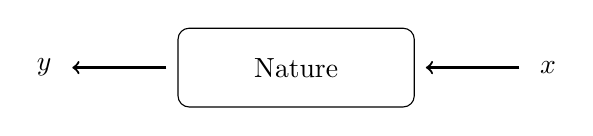
\begin{tikzpicture}[node distance=3.2cm, shorten >=4pt, ->]
        \tikzstyle{box} = [rectangle, rounded corners, minimum width=3cm, minimum height=1cm,text centered, draw=black, fill=white!100]
        \tikzstyle{arrow} = [thick, ->, shorten <= 4pt]
        
        \node (box) [box]{Nature};
        \node (y) [draw=none,fill=none, left of=box] {$y$};
        \node (x) [draw=none,fill=none, right of=box] {$x$};
        
        \draw [arrow] (x) -- (box);
        \draw [arrow] (box) -- (y);
    \end{tikzpicture}
\end{figure}
Inside the black box, nature associates the predictor variables with the response variables. We get to collect $y$ and $x$ as data, and the goal in analyzing them is twofold:
\begin{itemize}
    \setlength\itemsep{0cm}
    \item[] \textit{Understanding}. To extract some information about how nature is associating the response variables to the input variables
    \item[] \textit{Prediction}. To be able to predict what the responses are going to be when future inputs will be fed in
\end{itemize}
Similarly, there are two approaches towards these goals [\cite{Breiman2001}]:
\begin{itemize}
    \item \textit{The Data Modeling Culture}: The analysis starts by assuming a \textit{stochastic data model} for the inside of the black box, e.g. assuming that data are generated by independent draws from $y = f(x, \text{random noise}, \text{parameters})$, and then the values of the parameters are estimated from the data; model validation is performed based on goodness-of-fit tests and residuals analysis
    \item \textit{The Algorithmic Modeling Culture}: The analysis considers the inside of the box complex and unknown and the purpose is to find a function $f(x)$ -- an algorithm, a rule that operates on $x$ to predict the responses $y$; model validation is performed measuring predictive accuracy
\end{itemize}

These approaches differ in the logic used. The former start by trying to impose on nature a set of models -- often those the statisticians are comfortable with, well-known, whose properties are well studied -- and verifies that at least one of them is compatible with the data observed. The latter, on the contrary, is model-agnostic. Its ultimate target is finding \textit{a} rule that \textit{approximates} the mechanism associating inputs and outputs, even if this algorithm is convolute, inscrutable and unexpected, without imposing any a priori characteristics on the data-generating process. 

Breiman argues that statisticians in applied research consider data modeling as the main, if not the only, go-to for statistical analysis: 
\begin{displayquote}
    \say{I started reading the \textit{Annals of Statistics}, the flagship journal of theoretical statistics, and was bemused. Every article started with: \textit{Assume that the data are generated by the following model: ...}}
\end{displayquote}
The underlying assumption of the data modeling approach is that the parametric class of models imagined by the statistician for the complex mechanism devised by nature is indeed reasonable. Parameters are then estimated and conclusions are drawn. However, the conclusions drawn are about the model's mechanism, and not about nature's. Obviously, if the model is a poor approximation of nature, the conclusions may be wrong. On the other hand, a plus of data modeling is that it produces a simple and understandable description of the relationship between inputs and responses. This simplicity comes at the cost of uniqueness: different models, although equally valid, may give different descriptions of this relation. The fact that, following this approach, models are evaluated mainly using goodness-of-fit tests and other methods for checking fit, that yield a yes-no answer, creates difficulties in ranking the various models by quality [\cite{Breiman2001}]. The alternative proposed by the algorithmic culture is to measure the accuracy of the model's predictions: estimating the parameters in the model using the data and then using the model to predict the data checking how good the prediction is. The extent to which the model emulates nature's mechanics is a measure of how well the model can reproduce the natural phenomenon producing the data.

Sometimes approaching problems by looking for a data model imposes an a priori restriction to the ability of statisticians to deal with a wide range of statistical problems when they cannot be dealt with using models that remain enough understandable. The algorithmic community rarely make use of data models. Their approach starts by looking at the mechanics of how nature produces data as a black box partly unknowable. They stop at the mere acceptance of the fact that what is observed is a set of $x$'s that goes in and a set of $y$'s that comes out. The problem is rephrased as finding an algorithm, a rule $f(x)$, such that for future observed $x$, $f(x)$ will be a good predictor of $y$. The focus is shifted from data models to the properties of algorithms. The implicit assumption made in the theory is that the data is drawn $i.i.d.$ from an unknown multivariate distribution. The drawback of this approach is that models that best emulate nature in terms of predictive accuracy are also the most complex. 

Recent developments in both fields are trying to tie together these two cultures: this thesis goes in this direction, starting from the algorithmic approach and trying to extend it with concepts borrowed from the data modeling one. The philosophical underpinning throughout this work can be summarized as:
\begin{displayquote}
    The point of a model is to get useful information about the relation between the response and predictor variables. Interpretability is a way of getting information. But a model does not have to be simple to provide reliable information about the relation between predictor and response variables; neither does it have to be a data model. The goal is not interpretability, but accurate information [...] the emphasis needs to be on the problem and on the data -- \cite{Breiman2001}
\end{displayquote}
with a focus on the uncertainty regarding the information the model provides, i.e. its reliability in real life applications, that are the final purpose of all our efforts. Borrowing concepts from the Bayesian Nonparametric approach to statistics, we will try to construct the context around the algorithm. We will prove that any algorithm is a form of statistical modeling and that the separation from the two is not as clear-cut as Breiman suggests. That is why we will include algorithms into box of \textit{statistical modeling}.

How can we understand, concretely, the mechanics of nature? That depends on how nature manifests itself to us, namely what kind of data we are able to get. This shapes the way we can learn about nature from data and is the topic of the next section.




\section{Types of learning}\label{sec:types_of_learning}

All models, methods, techniques, algorithms, implemented to discover and understand the mechanics of nature are informally considered to perform a kind of leaning. This is true for any algorithm and, thus, also for neural networks. 

Therefore, neural networks can be viewed as a class of algorithms for statistical modeling and prediction. Based on a source of \textit{training data}, the aim is to produce a statistical model of the process, from which the data are generated: informally, we have to create a \say{story} for the data. Once we know the plot of the story, we can fill in the missing bits that the narrator has avoided telling us: what we call inference. We can distinguish three broad types of statistical modeling problems: \textit{density estimation}, \textit{classification} and \textit{regression}.

\textbf{Density estimation} problems are also referred to as \textbf{unsupervised learning} problems in the machine learning literature. In this class of problems, only the predictors are observed, no measurements of the outcome is provided. The learner's task is to describe how the data are organized or clustered, rather than make predictions [\cite{ESL}]. The goal is to model the unconditional distribution of data described by some vector $x$. 

\textbf{Classification} and \textbf{regression} problems are also referred to as \textit{supervised learning} problems in the machine learning literature. They only differ in the nature (discrete or continuous) of the target variable. In this class of problems we distinguish between \textit{input} variables, which we denote by $x$, and \textit{output} (or target) variables which we denote by the vector $y$. Classification problems require that each input vector $x$ be assigned to one of $K$ classes $\{y_1, \dots, y_K\}$ in which case the target variables represent class labels. Regression problems involve estimating the values of continuous variables $y$. Regression models and classification models both focus on the conditional density $p(y|x)$. Many regression techniques can be turned into classification methods by applying them to the problem of density estimation for the category probabilities. For example, if there are only two categories, we can denote them by $y \in \{0,1\}$. The regression problem is to model $E(y|x)$ that, thank to the definition of $y$, can be directly applied to the classification problem noting that $P(y = 1| x) = E[y|x]$. Hence, usually, any regression methods can be directly applied to classification [\cite{Lee2004}]. From the machine learning perspective, solving this class of problems entails learning an input-output mapping $f$ by examples: a function approximation task [\cite{ESL}]. This approximation, $f$, can be interpreted as, for example, $E(y|x)$.

Classification and regression problems can also be viewed as special cases of density estimation noting that the most general and complete description of the data is given by the probability distribution function $p(x,y)$ in the joint input-target space [\cite{Jordan1996}]. However, the usual goal is to be able to make good predictions for the target variables when presented with new values of the inputs. In this case it is convenient to decompose the joint distribution in the form:
$$p(x,y) = p(y|x) \; p(x)$$
and to consider only the conditional distribution $p(y|x)$. Seen in this form, it easy to assess how density estimation models can often arise more as components of the solution to a more general classification or regression problem -- since we may need an estimate of $p(x)$: to be able to estimate $p(x,y)$ or when there are missing data that we need to fill-in in a principled way. 

In what follows, we will focus on regression problems only: that is, the estimation of $p(y|x)$ from the data.





\section{The Anatomy of a Learner}
An informative high-level definition of learner, or learning algorithm, from a machine learning perspective is provided in \cite{Mitchell1997}:
\begin{displayquote}
    \say{A computer program is said to learn from experience \textit{E} with respect to some class of tasks \textit{T} and performance measure \textit{P}, if its performance at tasks in \textit{T}, as measured by \textit{P}, improves with experience \textit{E}}
\end{displayquote}
Of course, the variety of experiences, tasks, and performance measures is wide. Below a high-level overview of the possible instances of this concepts is provided:
\begin{itemize}
    \item Experiences \textit{E}: supervised or unsupervised learning
    \item Tasks \textit{T}: classification, classification with missing inputs, regression, anomaly detection, imputation of missing values, denoising, density estimation
    \item Performance measures \textit{P}: accuracy, error rate, goodness-of-fit tests
\end{itemize}
The starting point is the definition of a function approximator (or model). The statistician chooses an appropriate loss function according to the problem at hand. Once the loss function is chosen, an optimization criterion is defined, e.g. maximum likelihood, and an optimization routine must be set up. Typically the optimization problem is not solved analytically deriving a closed-form formula to provide a symbolic expression for the correct solution. On the contrary, updated estimates of the solutions are found via iterative processes\footnote{Optimization refers to the task of either minimizing or maximizing some function $J(\theta)$ by altering $\theta$. Since any maximization problem can be turned into a minimization problem, we will only consider minimization problems.}.

Therefore, all learning algorithms share a common \say{anatomy}:
\begin{enumerate}
    \item A specification of a dataset
    \item A model that defines a parametrised input-output mapping 
    \item A loss function that depends on the parameters of the model 
    \item An optimization procedure that finds the parameters values minimizing the loss function
\end{enumerate}
These components are modular: replacing them independently we can obtain a wide range of algorithms [\cite{Goodfellow-et-al-2016}]. The cost function typically includes at least one term that causes the learning process to perform statistical estimation. It may also include additional terms used for regularization.

This high-level description could be used for any algorithm as well as any statistical model! In the next section we will show that, in fact, they are two sides of the same coin. 





\section{Algorithms and Statistical models}
Given a dataset of pairs $\{y_i, x_i\}_{i=1}^{N}$, the simplest example of learning algorithm that can learn how to predict $y$ based on $x$ is linear regression. The underlying assumption is that the natural mechanics associating inputs and outputs can be described by a linear function mapping, $y = wx$. For each input-output pair, the model is a linear transformation of the inputs. Usually, a modified version of the model is used: an intercept term is added to the equation. This still preserves the linear mapping from parameters to predictions, but the mapping from features to predictions is now an affine function
$$y_i = w x_i + b$$
The intercept, in the machine learning literature, is often called the \textbf{bias}\footnote{This term is not related whatsoever to the idea of \textit{statistical bias}.} parameter (of the affine transformation) or \textbf{offset vector}. This nomenclature derives from the fact that, in the absence of any input, the transformation is biased towards $b$. 

Different parameters $w, b$ define different transformations. The goal is to find those values that minimize the errors in prediction, a procedure often referred to as \say{fitting} the model to data. There are many different methods to fit the model to data. To accomplish this task, the predictions are, thus, evaluated using a certain loss function. For continuous target variables the mean squared error (MSE) is often used: the values of $w$ and $b$ are chosen in a way that minimizes the residual sum of squares between the true outcomes and the predicted values.
$$\mathrm{MSE}(\theta) \stackrel{\scriptscriptstyle def}{=} J(\theta) = \sum_{i=1}^{N}\left\Vert y_i - (wx_i + b)\right\Vert_{2}^{2}, \quad \theta = (w,b)$$
where $\Vert\cdot\Vert$ is the $L^2$-norm (euclidean norm). The function $J$ will represent the \textit{loss} function henceforth, also called \textit{cost} or \textit{objective} function. Minimizing the loss function is the core of any machine learning algorithm. Therefore, there exists a tight relationship between learning and optimization. Optimizing a function requires being able to compute its derivative with respect to the parameters. 

Let's now build a story behind the algorithm. From a statistical point of view, we still assume that the true data-generating process can be described by a linear function mapping. However, in this case, we also assume that we are not able to observe the mechanics of nature directly: what we get to observe is a blurred picture of it. We call this \say{blurring} $\varepsilon$. We can, thus, rewrite the algorithm above as a statistical model where \say{statistical} comes from the fact that we are dealing with randomness. We collapse the intercept $b$ and $w$ into $\beta \stackrel{\scriptscriptstyle def}{=} (b, w)$, adding 1 as the first component of the vector of features, $x_i \stackrel{\scriptscriptstyle def}{=} (1, x_i)$. We make explicit an assumption often hidden when defining algorithms: our observations are independent and identically distributed. Thus we write
$$y_i = \beta x_i + \varepsilon_i \qquad \varepsilon \sim WN(0, \sigma^2)$$
where $WN$ stands for white noise. If we assume a specific parametric form for $WN$, e.g. a Gaussian distribution, we can write
$$y_i | x_i \stackrel{\scriptscriptstyle i.i.d.}{\sim} \mathcal{N}(\beta x_i, \sigma^2)$$
In this way we have defined a conditional probability $p(y|x)$. The toolbox of statistical inference contains various methods to estimate the parameter $\beta$ (and possibly $\sigma^2$). If, for example, we use the maximum likelihood approach, we would set the parameter to a value that maximizes the likelihood of our sample: again, we reduce inference (learning) to an optimization problem. In the Bayesian approach we would assign a prior to all uncertain quantities, in this case $\beta$, and use the Bayes' Theorem to compute the posterior of the parameters given the data.

We have now established a way to connect the two worlds and, strictly speaking, we have shown that what separates them is just the perspective from which we look at the problem. As soon as we assume that a certain degree of randomness exists, then we are in the realm of statistics. We thereby assert that for each algorithm there exists, perhaps not unique, a statistical interpretation.






\section{Neural Nets and Bayesian Nonparametrics}\label{sec:BNPreg}
Generally, the relation between $y$ and $x$ need not be linear. Indeed, in many interesting cases characterized by big and complex data (e.g. speech recognition, image processing) the mapping is better described by a nonlinear function. The regression model can be written in a general way as the combination of a deterministic regression function and a random residual
$$y = \underbrace{f(x)}_{\text{deterministic part}} + \underbrace{\varepsilon}_{\text{random part}}, \qquad \varepsilon \sim p_\varepsilon(\varepsilon)$$
As long as both, the regression function $f(\cdot)$ and the residual distribution $p(\cdot)$, are indexed by finitely many parameters, e.g. $(\beta, \sigma^2)$, inference reduces to a traditional parametric regression problem. The problem becomes a nonparametric regression when we wants to relax the parametric assumptions of either of the two model elements, that is the unknowns are not the parameters of a function, but the function itself.

Bayesian nonparametrics concerns Bayesian inference methods for \textit{nonparametric models}. A nonparametric model involves at least one infinite-dimensional parameter and hence may also be referred to as an \say{infinite-dimensional model}. Examples of infinite-dimensional parameters are functions or measures. The basic idea of nonparametric inference is to use data to infer an unknown quantity while making as few assumptions as possible. Usually, this means using statistical models that are infinite-dimensional. This characterization of nonparametric regression allows for three cases [\cite{MullerQuint2004}].

\paragraph{Nonparametric Residuals.} The model can be generalized by going nonparametric on the residual distribution, assuming $\varepsilon | G \stackrel{\scriptscriptstyle i.i.d.}{\sim} G$ with a nonparametric prior $p(G)$ on $G$, while keeping the regression mean function parametric as $f(\cdot) = f_\theta(\cdot)$  indexed by a (finite-dimensional) parameter vector $\theta$ with prior $p(\theta)$. We refer to this case as a \textit{nonparametric error model}. Essentially this becomes density estimation for the residual error. In principle, any model that is used for density estimation could be used. However, there is a minor complication. To maintain the interpretation of $\varepsilon$ as residuals and to avoid identifiability concerns, it is desirable to center the random $G$ at zero, for example, with $E(G) = 0$.

\paragraph{Nonparametric Mean Function.} One could, instead, relax the parametric assumption on the mean function and complete the model with a nonparametric prior $f(\cdot) \sim p(f)$. We refer to this as a \textit{nonparametric regression mean function}. Popular choices for $p(f)$ are Gaussian process priors [\cite{Rasmussen2006}] or priors based on basis expansions [\cite{Bishop2006}], regression trees [\cite{Breiman1984}], wavelet [\cite{vidakovic2009}], splines [\cite{Hastie1990, Denison}] or neural nets [\cite{Neal1996}]. Such methods can potentially approximate a wide range of regression functions. This approach, however, is  limited in the sense that it only allows for flexibility in the mean. Many datasets present non normality or multi-modality of the errors, degrees of skewness, or tail behavior in different regions of the covariate space. To capture such behaviors, a flexible approach for modeling the conditional density that allows both the mean and error distribution to evolve flexibly with the covariates is required.
    
\paragraph{Fully Nonparametric Regression.} One could go nonparametric on both assumptions. We refer to this as a \textit{fully nonparametric regression}. The sampling model becomes $p(y_i | x_i) = G_x$, with a prior on the family of \textit{conditional random probability measures}, $p(G_x, x \in \mathrm{X})$. Many commonly used priors for $\mathcal{G} = \{G_x\}$ are variations of dependent Dirichlet Process priors [\cite{Maceachern1999}].


\bigbreak

Although limited for the reasons we mentioned above, the \textit{nonparametric regression mean function} is a powerful tool, especially with the implementation of deep neural nets -- possible thanks to the advent of modern computers and the development of further numerical methods and software packages, e.g. \texttt{PyTorch} and \texttt{TensorFlow}. Usually, the residuals are assumed iid Gaussian with mean zero and with common variance. If this is the case, i.e. $\varepsilon$ has zero mean, then $f(x) = \mathrm{E}(y|x)$ becomes the \textit{conditional mean function}. When the assumption of a straight line (or a hyperplane) fit may be overly restrictive we may think to use a richer class of functions. The typical nonparametric regression model is of the form
$$y_i = f(x_i) + \varepsilon_i$$
where $f\in\mathcal{F}$, some class of regression functions. Nonparametric regression models differ in the class of functions to which $f$ is assumed to belong. The exist a variety of different ways to choose $\mathcal{F}$. There exist two classes that are very close to neural networks: local methods and basis functions.

\paragraph{Local methods.} These are some of the simplest approaches to nonparametric regression that operate locally. For example, in one dimension a moving average with a fixed window size would result in a step function. Sophistication can be added in the choice of the window, the weighting of the averaging, or the shape of the fit over the window. One example of such sophistication is \textit{kernel smoothing}: the idea is to use a moving weighted average, where the weight function is referred to as a kernel. A kernel is a continuous, bounded, symmetric function whose integral is one. Whatever the choice of the kernel, the resulting regression function estimate at a value $x$ of a single explanatory variable is 
$$\hat{y} = \frac{\sum_{i=1}^{n} y_i K(x-x_i)}{\sum_{i=1}^{n} K(x-x_i)}$$
The kernel regression approach is intertwined with work on kernel density estimation [\cite{Silverman1986, Loader2006}]. Kernels can be generalized to multiple dimensions, but data sparseness quickly becomes an issue. 

A completely different approach is to abandon the moving window in favour of partitioning the space into an exhaustive set of mutually exclusive regions. Using a constant function over the region gives rise to a step function. In one dimension, this is a histogram estimator [\cite{Gentle2002}, section 9.2]. In higher dimensions, a tree is a useful method for representing the splitting of the space into regions [\cite{Breiman1984}]. For regression, the predicted value is the average value of the response variable in a region, and for classification the fitted probability of class membership is the empirical probability in that region. 

\paragraph{Basis functions.} A large class of nonparametric methods are those that use an infinite set of basis functions to span the space of interest, e.g. $\mathcal{F}$ -- typically either the space of continuous functions or the space of square-integrable functions. The regression model becomes of the form
$$y_i = \sum_{k = 0}^{\infty} \beta_k \phi_k(x_i) + \varepsilon_i$$
where $\phi_1, \phi_2, \dots$ is a set of basis functions and, usually, $\phi_0$ is defined equal to 1 everywhere. 
An infinite number of terms would typically be required for a theoretical match to a continuous function, but in practice a finite number of terms is used to provide a close approximation to the infinite sum. We can obtain this imposing $k = 1,\dots,K$ and then to form a linear combination of these functions, so that for a sufficiently large value of $K$, and for a suitable choice of the $\phi_k(x)$, such a model has the desired \say{universal approximation} properties. Models of this form have the property that they
can be expressed as network diagrams in which there is a single layer of adaptive weights, also called \textbf{shallow learners} in the machine learning literature [\cite{Polson2017}].

An example of a basis set that spans the space of continuous functions is the standard basis of the vector space of all polynomials, $\{1, x, x^2, x^3, x^4, \dots\}$. Any continuous function can be approximated arbitrarily closely with a linear combination of these functions. Also mixture models can be basis representations, depending on the particular form of the model. One common form of a mixture model is the mixture of Gaussians: a collection of Gaussian densities is used as a basis set. For a univariate problem the model is
$$y_i = \sum_{k=0}^{\infty}\beta_k \phi\left(\frac{x_i - \mu_k}{\sigma_k}\right) + \varepsilon_i$$
where $\phi(u) = \frac{1}{\sqrt{2\pi}}\exp\{-u^2/2\}$ is the standard Gaussian density function, and $\mu_k$ and $\sigma_k$ are, respectively, the mean and standard deviation of the Gaussians in the mixture.


\section{Neural Networks}
We can now, naturally, introduce neural networks in the context of nonparametric regression. Neural networks are a particular case of basis function in which the basis functions are defined as $\phi_k^{w, b}(x) = \varphi(w_k x + b_k)$, where the scalar-valued nonlinear function, $\varphi$, is applied to the affine transformation of the inputs. The nonlinearity, also called \textbf{activation function}, is defined to be identical for all inputs. The most common activation function used are presented in figure \ref{fig:activation_functions}. The intermediate layer is called \textbf{hidden layer}. The dimesionality, $K$, of the hidden layer defines the \textbf{width} of the model, while the overall number of hidden layers determines the \textbf{depth} of the model -- being a plain neural network the depth is obviously one. 
\begin{figure}[ht]
    \centering
    \includegraphics[width=\textwidth]{images/activations.png}
    \caption{Most used activation functions.}
    \label{fig:activation_functions}
\end{figure}
Usually, layers are not interpreted as vector-to-vector functions. Rather, they are thought of as consisting of computational units or neurons, that act in parallel, each representing a vector-to-scalar function. This view highlights the inspiration of neural networks to the human brain. The univariate model can be written as
$$y_i = \sum_{k=0}^{K} \beta_k \; \phi_k^{w, b}(x) + \varepsilon_i$$
\begin{figure}
    \centering
    \includegraphics[scale=0.4]{images/nn.jpg}
    \caption{A stylized example of a fully-connected feedforward neural network. The input layer has four units, corresponding to the components of the vector $x_i \in \mathbb{R}^Q, \; i = 1,\dots, N$, with $Q = 4$. Each circle is a neuron calculates a weighted sum of an input vector plus bias and applies a nonlinear function to produce an output, which is this case is a scalar $y_i, \; i=1,\dots,N$, that is $D = 1$.}
    \label{fig:neural_network}
\end{figure}
This is the canonical example of neural network, known also as fully-connected feedforward neural network [\cite{Rosenblatt1958, Goodfellow-et-al-2016}]. Note that in the machine learning literature the basis functions are called \textit{hidden nodes}. For a historical review of neural networks and deep learning consult \cite{Schmidhuber2015}. 

It can be interpreted as a two-stage regression model: in the first stage the features are derived via a composition of an affine transformation of the inputs and a component-wise nonlinear function. These extracted features, in the second stage, are mapped to the output via a second affine transformation [\cite{ESL}]. In fact, also linear regression can be interpreted as a very simple example of neural network where $\varphi$ is an identity mapping. These models are associated with directed acyclic graphs, known as \textit{network diagram}. The neural network described above can be represented as in figure \ref{fig:neural_network}. To extend the above model to a multivariate $y$, we simply treat each dimension of $y$ as a separate output and add a set of connections from each hidden node to each of the dimensions of $y$. We can also assign an observation-specific residual variance.

It is clear from the equation above  that a (deep) neural network is simply a nonparametric regression using a basis representation. In other words, the key to understanding a neural network model is to think of it in terms of basis functions. 

From the equation above, it is also clear that a neural network is a standard parametric model, with a likelihood and parameters to be fit. We can, thus, claim that it is not a black box or purely an algorithm. It should now be apparent that neural nets are both algorithms \textit{and} statistical models. By viewing neural networks as statistical models, we can now apply many other ideas in statistics in order to understand, improve, and appropriately use these models. The disadvantage of viewing them as algorithms is that it can be difficult to apply knowledge from other algorithms. Taking the model-based perspective, we can be more systematic in discussing issues such as choosing a prior, building a model, checking assumptions for the validity of the model, and understanding uncertainty in our predictions [\cite{Lee2004, Polson2017}]. 

The neural network described above is an example of a shallow learner: informally, every model that cannot be categorized as deep is a shallow learner. Almost all shallow learners are data reduction techniques that consist of a low dimensional auxiliary variable $Z$ and a prediction rule specified by a composition of functions
$$f(x) = f_2\big(f_1(x)\big) = f_2(z), \qquad f_1(x) \coloneqq z$$
\begin{figure}[ht]
    \centering
    \includegraphics[scale=0.06]{images/nn_lr.png}
    \caption{The network graph of linear regression. For each observation, the predictor is a 3-D vector. The addition of the intercept has been made explicit.}
    \label{fig:lr_neural_network}
\end{figure}
Linear regression, Logistic regression, Principal component analysis, Partial least squares, Reduced rank regression, Linear discriminant analysis and Project pursuit regression are all examples of shallow learners. Furthermore, they all can be represented as a neural network, for example a linear regression network diagram is shown in figure \ref{fig:lr_neural_network}.



\section{Neural Nets as Graphical Models}
How can we represent conditional and unconditional distributions with neural networks? One way to answer this question is to find a suitable graph representation of probability distributions. Probabilistic Graphical Models (PGM) use diagrammatic representations to describe random variables and relationships among them. Similar to a graph that contains nodes (vertices) and links (edges), PGM has nodes to represent random variables and links to express probabilistic relationships among them. Below we will provide a simple example.

Consider a case in which we want to model the unconditional distribution $p(x)$. A general approach to density estimation is to treat the density as being composed of a set of $K$ simpler densities, where possibly $K=\infty$. This approach is a probabilistic form of clustering which involves modeling the observed data as a sample from a \textit{mixture density}:
$$p(x|\pi) = \sum_{i=1}^{K} \pi_i \; p(x|i, \theta_i)$$
where the $\pi_i$ are constants known as \textit{mixing proportions}, the $p(x|i, \theta_i)$ are the \textit{component densities}, generally taken to be from a simple parametric family, and $\theta_i$ are the parameters of the component densities. A common choice for component density is the multivariate Gaussian. In this case $\theta_i = (\mu_i, \Sigma_i)$. By varying this parameter, a wide variety of high-dimensional, multi-modal data can be modeled. Gaussian mixtures are representable as simple networks with one or more layers of adaptive weights, e.g. principal component analysis, canonical correlation analysis, kernel density estimation and factor analysis [\cite{Polson2017}], as shown in fig. \ref{fig:gaussianmix}. 
\begin{figure}
    \centering
    \includegraphics[scale=0.5]{images/gaussianmix.png}
    \caption{A network representation of a Gaussian mixture distribution. The input nodes representing the components of $x$ are in the lower level. Each link has a weight $\mu_{ij}$, which is the $j$-th component of the mean vector for the $i$-th Gaussian. Each node in the intermediate layer contains the covariance matrix $\Sigma_i$ and computes the Gaussian conditional probability $p(x|i,\mu_i,\Sigma_i)$. These probabilities are weighted by the mixing proportions $\pi_i$ in the last layer and the output node calculates the weighted sum $p(x) = \sum_i \pi_i p(x|i, w_i)$.}
    \label{fig:gaussianmix}
\end{figure}
Neural networks express relationships between variables by utilizing the representational language of graph theory. Variables are associated with nodes in a graph and transformations of variables are based on algorithms that \say{[...] propagate numerical messages along the links of the graph} [\cite{Jordan1996}]. The graphs is accompanied by probabilistic interpretations of the variables and their interrelationships. As we have seen, such probabilistic interpretations allow a neural network to be understood as a form of probabilistic model and reduce the problem of learning the weights of a network to a problem in statistics. Hidden Markov models and Dynamic Linear models -- also called Kalman filters in the machine learning literature -- are all examples of graphical probabilistic models. There is a strong relationship between these models and neural networks: it is often possible to reduce one kind of model to the other. Indeed, neural networks can be seen as members of a general family of probabilistic graphical models [\cite{Goodfellow-et-al-2016}, ch. 20].

Although elegant, this interpretation of the neural nets is limited since interpretability becomes easily an issue when the network grows deep. That is why it will not be treated in what follows. A more useful interpretation, is to look at neural nets as a highly nonlinear nonparametric function approximator, that is as a particular case of basis function.


\section{Deep Learners and Deep Neural Networks}
Deep learning refers to a wide class of machine learning techniques and architectures, with the common trait of \say{[...] using many layers of nonlinear information processing} [\cite{DengYu2014}]. In general, a deep learner, is a representation learning methods with multiple levels of representation, obtained by composing simple but nonlinear transformations of the raw data, with each of these transforming the representation at one level (starting with the raw input) into a representation at a higher level of abstraction. Composing enough of such transformations, very complex functions can be learned [\cite{LeCun2015}]. A deep architecture can be thought as a multilayer stack of simple models.

A \textbf{Deep Neural Net} (DNN) simply applies a composition of functions $\phi$, instead of a single one. Deep neural nets provide a flexible representations of $f(\cdot)$ capable of rendering nonlinear mappings which can approximate any given mapping to arbitrary accuracy. Given an input, $X \in \mathbb{R}^Q$, and an output, $Y \in \mathbb{R}^D$, usually both high-dimensional, the mapping $f: {R}^Q \rightarrow {R}^D$ is modeled via the superposition of univariate semi-affine functions where univariate activation functions are used to decompose the high-dimensional $X$, as a plain neural network. The particular characteristic of DNN is the depth of the networks, usually more than 2 hidden layers. Then a deep prediction rule can be expressed, in matrix notation, as:
\begin{align*}
    h^{(1)} &= \varphi_1 \left( W^{(0)}X + b_{0}\right)\\
    h^{(2)} &= \varphi_2 \left( W^{(1)}  h^{(1)} + b_{1}\right)\\
    &\cdots\\
    h^{(L)} &= \varphi_L \left( W^{(L-1)} h^{(L-1)} + b_{L-1}\right)\\
    f(X) &= W^{(L)} h^{(L)} + b_{L}
\end{align*}
where $h^{(l)}$ identifies the layer and the $\beta_k$'s have been collapsed in the matrix $W$, for each layer. DNN are, perhaps, the most famous inhabitant of this class of models in recent years, however other models characterized by deep architecture exists: deep gaussian processes [\cite{Damianou2013, Lee2017}] and neural processes [\cite{Garnelo2018a}] that are treated in the following chapters.

How a series of simple operation can represent complicated mappings? In other words, why this approach works? The formal roots of DL can be traced back in Kolmogorov's representation of a multivariate response surface as a superposition of univariate activation functions applied to an affine transformation of the input variables [\cite{Kolmogorov1957}]. In 1957 the Russian mathematician Kolmogorov showed that \textit{any} continuous function $f$ of many variables can be represented as a composition of addition and
some functions of one variable. The original version of this theorem can be expressed as follows\footnote{We propose a version of the theorem deducted from \cite{Kolmogorov2009, Kolmogorov2011}.}:
\begin{theorem}[Kolmogorov–Arnold superposition theorem]
    Let $f: [0, 1]^{d} \rightarrow \mathbb{R}$ be an arbitrary multivariate continuous function defined on the identity hypercube. Then it
has the representation 
$$f(\mathbf{x}) = f(x_1, \dots, x_d) = \sum_{q=0}^{2d} \phi_q \left(\sum_{p=1}^{d} \psi_{q,p} (x_p) \right)$$
with continuous one–dimensional inner and outer functions $\phi_q$ and $\psi_{q,p}$, defined on the real line. The inner functions $\psi_{q,p}$ are independent of the function $f$.
\end{theorem}
Starting from the 2000s, Kolmogorov’s superposition theorem found the attention of the machine learning community interest in providing a theoretical justification of neural networks. Hecht–Nielsen’s [\cite{Kolmogorov2011}] tries to apply the theorem to a feed-forward network with an input layer, one hidden layer and an output layer [\cite{Kolmogorov1987}]. However, the inner functions, $\psi$, in this application of the theorem are highly nonsmooth and thus not useful in optimization. Sprecher [\cite{Kolmogorov1965}] contributed to this research topic providing an explicit method to construct the univariate functions $\psi$, corresponding to the activation functions of the network. Bryant [\cite{Bryant2008}] implements Sprecher's [\cite{Kolmogorov1972}] algorithm to estimate the inner link function. In his application of the theorem, deep layers allow for smooth activation functions to provide \say{learned} hyperplanes which find the underlying complex interactions and regions without having to see an exponentially large number of training samples.

To summarize, deep learning architectures rather than manually engineering the transformations to be applied to create more abstract concepts, learn them: the behaviour of the hidden layers is not directly specified in the data, it is learned. 











